\chapter{Polar Coordinates, Vectors and Complex Numbers}
\author{Nithin}

\section{Polar Coordinates}
\begin{figure}
    \centering
    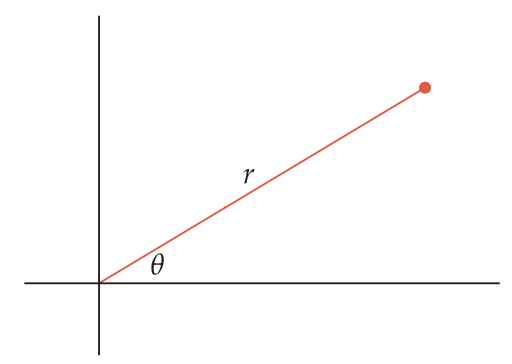
\includegraphics[width=0.5\textwidth]{polar1.png}
\end{figure}
The polar coordinates of a point in the plane are given by the ordered pair \((r, \theta)\), where:
\begin{itemize}
    \item \(r\) is the distance from the point to the origin (the pole).
    \item \(\theta\) is the angle measured from the positive x-axis to the line connecting the point to the origin.
\end{itemize}

\subsection{Polar to Rectangular Coordinates}
\begin{figure}
    \centering
    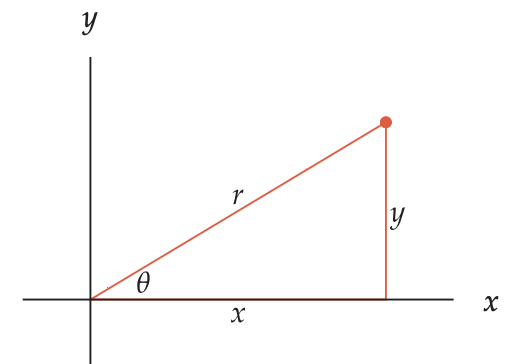
\includegraphics[width=0.5\textwidth]{polar2.png}
\end{figure}
The conversion from polar coordinates \((r, \theta)\) to rectangular coordinates \((x, y)\) is given by:
\[ x = r \cos(\theta), \quad y = r \sin(\theta) \]
The conversion from rectangular coordinates \((x, y)\) to polar coordinates \((r, \theta)\) is given by:
\[ r = \sqrt{x^2 + y^2}, \quad \theta = \tan^{-1}\left(\frac{y}{x}\right) \]

\subsection{Ambiguity in Polar Coordinates: Case 1}
Find polar coordinates for the point \((1, 1)\):
\begin{figure}
    \centering
    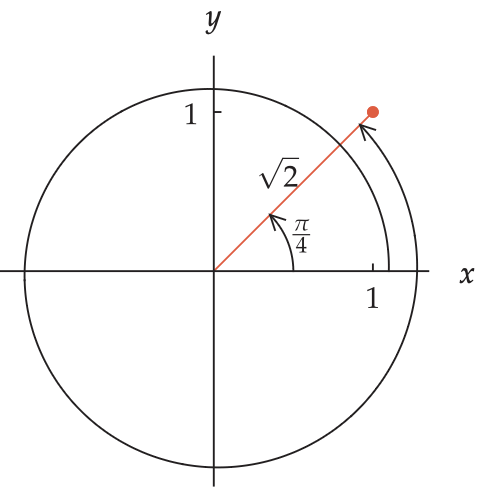
\includegraphics[width=0.5\textwidth]{polar3.png}
\end{figure}
\begin{itemize}
    \item \(r = \sqrt{2}, \theta = \frac{\pi}{4}\)
    \item Polar coordinates are not unique. For example, the point at \( (\sqrt{2}, \frac{\pi}{4}) \) can also be represented as \( (\sqrt{2}, \frac{\pi}{4} + 2k\pi) \)  for any integer \( k \).
\end{itemize}

\subsection{Ambiguity in Polar Coordinates: Case 2}
Find polar coordinates for the point \((1, -1)\):
\begin{figure}
    \centering
    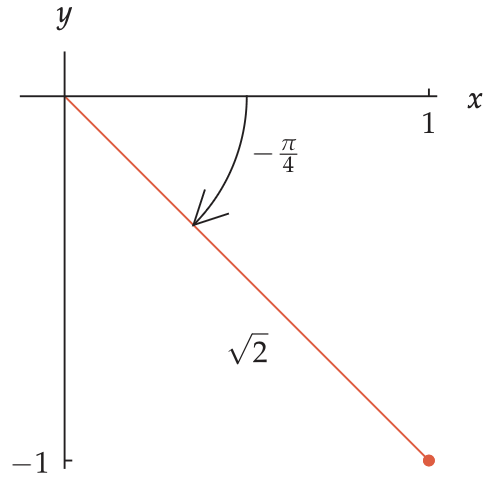
\includegraphics[width=0.5\textwidth]{polar4.png}
\end{figure}
\begin{itemize}
    \item \(r = \sqrt{2}, \theta = -\frac{\pi}{4}\)
    \item The point can also be represented as \( (\sqrt{2}, -\frac{\pi}{4} + 2k\pi) \) for any integer \( k \).
\end{itemize}

\subsection{Ambiguity in Polar Coordinates: Case 3}
Find polar coordinates for the point \((-1, 1)\):
\begin{figure}
    \centering
    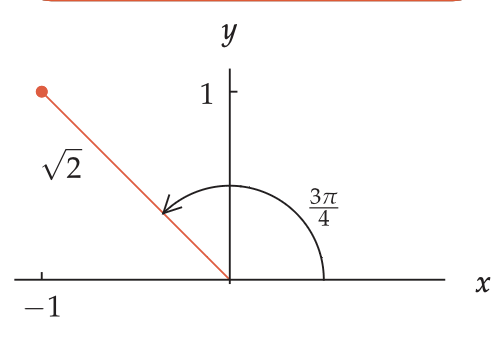
\includegraphics[width=0.5\textwidth]{polar5.png}
\end{figure}
\begin{itemize}
    \item \(r = \sqrt{2}, \theta = \tan^{-1} \left(\frac{1}{-1}\right) = -\frac{\pi}{4}\)
    \item For the above polar co-ordinates the point is \((1,-1)\) not \((-1, 1)\).
    \item From the figure the correct choice is \(\frac{3\pi}{4}\) or \(\frac{3\pi}{4} + 2k\pi\) for any integer \( k \).
    \item arctan failed in this case because the point is in the second quadrant while arctan is defined only for the first and fourth quadrants.That is \((\frac{\pi}{2},\frac{-\pi}{2})\)
\end{itemize}

\subsection{Converting Polar Coordinates to Rectangular Coordinates}
A point with rectangular coordinates \((x, y)\), with \(x \neq 0\) has polar coordinates \(r,\theta\) that satisfy the equations
\begin{align*}
    r = \sqrt{x^2 + y^2} \\
    \tan(\theta) = \frac{y}{x}
\end{align*}
where \(\theta\) must be chosen so that \(\cos \theta \) has the same sign as \(x\) and \(\sin \theta\) has the same sign as \(y\).

\subsection{Exercise}
Find the polar co-ordinates for the point with rectangular coordinates \((-3, 4)\).
Solution:
\begin{align*}
    r &= \sqrt{(-3)^2 + 4^2} = \sqrt{9 + 16} = \sqrt{25} = 5 \\
    \theta &= \tan^{-1}\left(\frac{4}{-3}\right) = \tan^{-1}\left(-\frac{4}{3}\right) + \pi
\end{align*}

\subsection{Graphs of Polar Equations}
\subsubsection{Circle}
If \(C\) is a positive number, then the polar equation \(r = C\) represents a circle centered at the origin with radius \(C\).
\subsubsection{Ray}
If \(C\) is a real number, Then polar equation \(\theta = C\) represents a ray starting from the origin at angle \(C\).

\section{vectors}
\subsection{What is a Vector?}
A vector is a quantity that has both magnitude and direction. Vectors are often represented graphically as arrows.
\begin{itemize}
    \item The length of the arrow represents the magnitude of the vector.
    \item The direction of the arrow indicates the direction of the vector.
    \item Two vectors are equal if they have the same magnitude and direction, regardless of their position in space.
\end{itemize}

\subsection{Points vs. Vectors: Notation}
If \(a\) and \(b\) are real numbers, then \((a, b)\) can denote either a point or a vector, depending on the context:
\begin{itemize}
    \item \textbf{Point:} The point in the coordinate plane whose first coordinate is \(a\) and whose second coordinate is \(b\).
    \item \textbf{Vector:} The vector whose initial point is the origin and whose endpoint has first coordinate \(a\) and second coordinate \(b\).
\end{itemize}
It is important to distinguish between these two uses based on context.
\begin{figure}
    \centering
    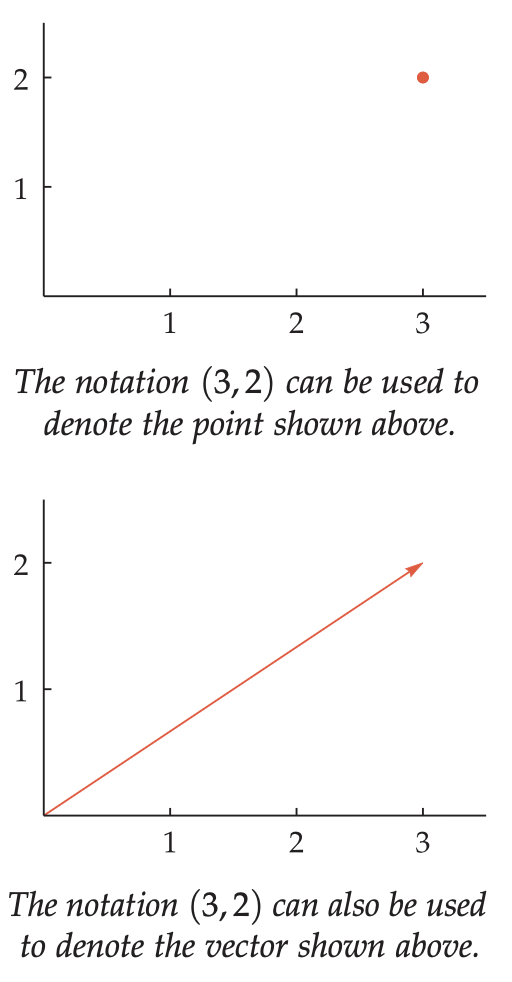
\includegraphics[width=0.3\textwidth]{vector1.png}
    \caption{Vector Representation}
    \label{fig:vector_representation}
\end{figure}

\subsection{Magnitude and Direction of a Vector}
Suppose a vector \(\vec{u}\) is positioned so that its initial point is at origin. If the endpoint of \(\vec{u}\) has polar coordinates \((r, \theta)\)
\begin{itemize}
    \item the magnitude of \(\vec{u}\) is given by \(r\).
    \item the direction of \(\vec{u}\) is given by \(\theta\).
\end{itemize}
\begin{figure}
    \centering
    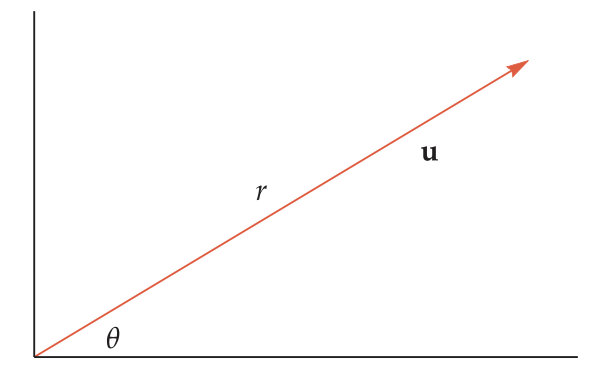
\includegraphics[width=0.3\textwidth]{vector2.png}
    \caption{Vector with Magnitude and Direction}
    \label{fig:vector_magnitude_direction}
\end{figure}

\subsection{Computing the Magnitude and Direction of a Vector}
if \(\vec u = (a,b)\) then
\begin{itemize}
    \item \(|u| = \sqrt{a^2 + b^2}\)
    \item An angle \(\theta\) that determines the direction of \(\vec{u}\) satisfies the equation \(\tan \theta = \frac{b}{a}\), where \(\theta\) must be chosen so that \(\cos \theta\) has the same sign as \(a\) and \(\sin \theta\) has the same sign as \(b\).
\end{itemize}

\subsection{Vector Addition}
\begin{itemize}
\item If the endpoint of a vector \(\vec u\) coinicides with the initial point of a vector \(\vec v\), then the vector \(\vec u + \vec v\) has the same initial point as \(\vec u\) and the same endpoint as \(\vec v\).
\item If \(u = (a,b)\) and \(v = (c,d)\), then \(\vec u + \vec v = (a+c, b+d)\).
\end{itemize}
\begin{figure}
    \centering
    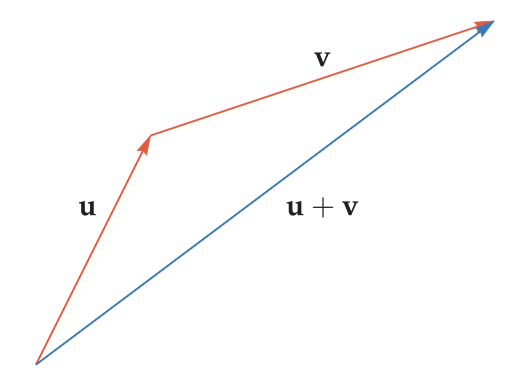
\includegraphics[width=0.4\textwidth]{vector3.png}
    \caption{Vector Addition}
    \label{fig:vector_addition}
\end{figure}

\subsection{Vector Addtition: Commutative and Associative Properties}
\begin{itemize}
    \item Vector addition is commutative: \(\vec u + \vec v = \vec v + \vec u\)
    \item Vector addition is associative: \((\vec u + \vec v) + \vec w = \vec u + (\vec v + \vec w)\)
\end{itemize}
\begin{figure}
    \centering
    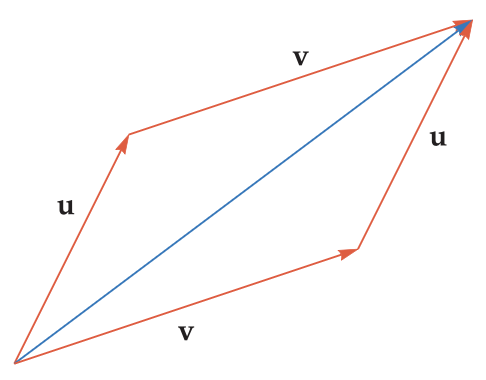
\includegraphics[width=0.4\textwidth]{vector4.png}
    \caption{Vector Addition Properties}
    \label{fig:vector_subtraction}
\end{figure}

\subsection{Vector Subtraction}
\subsubsection{Additive Inverse}
\begin{itemize}
    \item If \(\vec u \) is a vector, then the vector \(-\vec u\) is called the additive inverse of \(\vec u\). The vector \(-\vec u\) has the same magnitude as \(\vec u\) but points in the opposite direction
    \item If \(\vec u\) has polar coordinates \((r, \theta)\), then the polar coordinates of \(-\vec u\) are \((r, \theta + \pi)\).
    \item If \(\vec u = (a,b)\), then \(-\vec u = (-a,-b)\).
\end{itemize}

\subsection{Scalar Multiplication of Vectors}
Suppose \(t\) is a real number and \(\vec{u}\) is a vector.
\begin{itemize}
    \item The vector \(t\vec{u}\) has magnitude \(|t|\) times the magnitude of \(\vec{u}\); that is, \(|t\vec{u}| = |t||\vec{u}|\).
    \begin{itemize}
        \item If \(t > 0\), then \(t\vec{u}\) has the same direction as \(\vec{u}\).
        \item If \(t < 0\), then \(t\vec{u}\) has the opposite direction of \(\vec{u}\).
    \end{itemize}
    \item Suppose \(\vec{u}\) has polar coordinates \((r, \theta)\).
    \begin{itemize}
        \item If \(t > 0\), then \(t\vec{u}\) has polar coordinates \((tr, \theta)\).
        \item If \(t < 0\), then \(t\vec{u}\) has polar coordinates \((|t|r, \theta + \pi)\).
    \end{itemize}
    \item If \(\vec{u} = (a, b)\), then \(t\vec{u} = (ta, tb)\).
\end{itemize}

\subsection{Dot Product}
The dot product of two vectors \(\vec{u} = (a, b)\) and \(\vec{v} = (c, d)\) is defined as:
\[ \vec{u} \cdot \vec{v} = ac + bd \]
\begin{itemize}
    \item The dot product is a scalar quantity.
    \item Geometrically, the dot product can be expressed in terms of the magnitudes of the vectors and the cosine of the angle \(\theta\) between them:
    \[ \vec{u} \cdot \vec{v} = |\vec{u}||\vec{v}|\cos\theta \]
\end{itemize}

\subsection{Algebraic Properties of the Dot Product}
\begin{itemize}
    \item Commutative Property: \(\vec{u} \cdot \vec{v} = \vec{v} \cdot \vec{u}\)
    \item Distributive Property: \(\vec{u} \cdot (\vec{v} + \vec{w}) = \vec{u} \cdot \vec{v} + \vec{u} \cdot \vec{w}\)
    \item Scalar Multiplication: \((k\vec{u}) \cdot \vec{v} = k(\vec{u} \cdot \vec{v})\) for any scalar \(k\)
    \item Identity Property: \(\vec{u} \cdot \vec{u} = |\vec{u}|^2\)
\end{itemize}

\subsection{Geometric Interpretation of the Dot Product}
\begin{itemize}
    \item The dot product \(\vec{u} \cdot \vec{v}\) can be interpreted geometrically as a measure of how much one vector extends in the direction of another.
    \item If \(\theta\) is the angle between \(\vec{u}\) and \(\vec{v}\), then:
    \[ \vec{u} \cdot \vec{v} = |\vec{u}||\vec{v}|\cos\theta \]
    \item This means that the dot product is maximized when the vectors are in the same direction (\(\theta = 0\)) and minimized when they are orthogonal (\(\theta = 90^\circ\)).
\end{itemize}
\begin{figure}
    \centering
    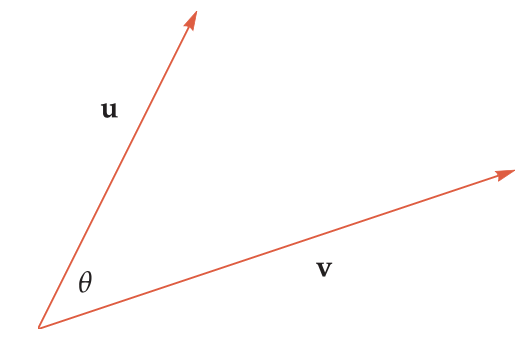
\includegraphics[width=0.3\textwidth]{vector5.png}
    \caption{Geometric Interpretation of the Dot Product}
    \label{fig:dot_product}
\end{figure}

\subsection{Geometric Interpretation of the Dot Product: Proof}
\begin{align*}
    | \vec{u} - \vec{v}|^2 &= (\vec{u} - \vec{v}) \cdot (\vec{u} - \vec{v}) \\
    &= \vec{u} \cdot (\vec{u} - \vec{v} ) - \vec{v} \cdot (\vec{u} - \vec{v}) \\
    &= \vec{u} \cdot \vec{u} - \vec{u} \cdot \vec{v} - \vec{v} \cdot \vec{u} + \vec{v} \cdot \vec{v} \\
    &= |\vec{u}|^2 - 2\vec{u} \cdot \vec{v} + |\vec{v}|^2 \\
    &= |\vec{u}|^2 + |\vec{v}|^2 - 2\vec{u} \cdot \vec{v}
\end{align*}
\begin{figure}
    \centering
    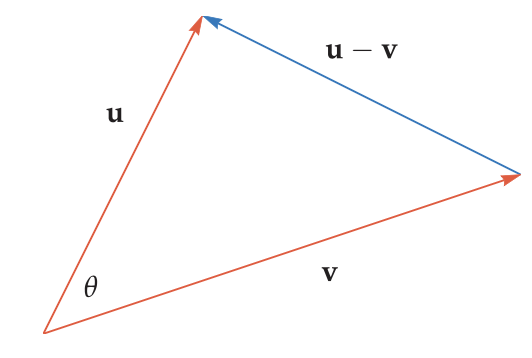
\includegraphics[width=0.2\textwidth]{vector6.png}
    \caption{Geometric Interpretation of the Dot Product: Proof}
    \label{fig:dot_product_proof}
\end{figure}
Using the law of cosines
\begin{align*}
    |\vec{u} - \vec{v}|^2 &= |\vec{u}|^2 + |\vec{v}|^2 - 2|\vec{u}||\vec{v}|\cos\theta \\
    |\vec{u}|^2 - 2\vec{u} \cdot \vec{v} + |\vec{v}|^2 &= |\vec{u}|^2 + |\vec{v}|^2 - 2|\vec{u}||\vec{v}|\cos\theta \\
    \vec{u} \cdot \vec{v} &= |\vec{u}||\vec{v}|\cos\theta
\end{align*}

\subsection{Perpendicular Vectors}
Two vectors \(\vec{u}\) and \(\vec{v}\) are said to be perpendicular (or orthogonal) if their dot product is zero:
\[ \vec{u} \cdot \vec{v} = 0 \]
\begin{itemize}
    \item Geometrically, this means that the angle \(\theta\) between the vectors is \(90^\circ\).
    \item If \(\vec{u} = (a, b)\) and \(\vec{v} = (c, d)\), then the condition for perpendicularity can be expressed as:
    \[ ac + bd = 0 \]
\end{itemize}

\section{Complex Numbers}
\subsection{Why Complex Numbers?}
\begin{itemize}
    \item The real number system provides a powerful context for solving a broad array of problems.
    \item Calculus takes place mostly within the real number system.
    \item However, some important mathematical problems cannot be solved within the real number system.
    \item Complex numbers extend the idea of one-dimensional number lines to two dimensions.
    \item They are useful in representing and solving problems in physics, engineering, and applied mathematics.
    \item The complex plane allows for a geometric interpretation of complex numbers.
\end{itemize}
